%%=============================================================================
%% Inleiding
%%=============================================================================

\chapter{Inleiding}
\label{ch:inleiding}

Security is de laatste jaren een echte trend geworden. Elk bedrijf is hiermee bezig, en ook in het nieuws komen er steeds meer berichten over beveiliging. Maar hoe zou een bedrijf hier zich best tegen kunnen verdedigen? Is een gewone firewall en antivirus niet genoeg meer?

%TODO: termen vulnerability & exploit &C VE uitleggen?

De volgende stap is voor vele bedrijven een 'Vulnerability management' systeem. Dit is een continu proces dat bestaat uit 4 delen:  'discovery', 'reporting', 'prioritization' en 'response'. Tijdens het 'discovery' deel moet ELK systeem getest worden en in een databank geplaatst worden. Deze databank wordt gebruikt in de volgende stap 'reporting'. Hier moet er een rapport gemaakt worden zodat alle risico's in kaart gebracht kunnen worden. Eens dat de rapporten klaar zijn, moeten er 'priorities' opgesteld worden. Dit gebeurt door elk risico te bekijken en studeren wat de invloed is op het netwerk als deze misbruikt word. Uiteindelijk moeten deze risico's opgelost worden in het 'response' deel. \textcite{Tripwire}

%TODO: laatste wworden als SQL injecties enzo uitleggen?
Tools dat hiervoor gebruikt kan worden zijn noemen we scanners. In deze bachelorproef zal ik alleen de 'Vulnerability scanners' bespreken. Dit is een beveiligingstechniek  dat fouten in een systeem kan opsporen \textcite{Techopedia} over een netwerk. Deze tools worden zowel gebruikt door 'black hats' als 'white hats'. Het verschil tussen deze 2 is dat de 'white hat' ethisch correct is. Deze zal op voorhand toegang vragen om een systeem te mogen testen, en als deze test lukt het bedrijf melden wat er mis is. De 'black hat' vraagt geen toestemming en gebruikt de testen om binnen te dringen op een systeem en de data hiervan te verkopen, of het systeem te laten crashen \textcite{Howtogeek}. Voor een volledig vulnerabiliy management bij te houden, moet men ook nog andere scanners implementeren zoals een 'web application scanner' (bv. Arachni). Deze scant een website op mogelijke problemen als SQL injecties en cross-site scripting.

%TODO: complexe formule erbij zetten? + NOG BIJZETTEN OP EINDE OVER CVE'S EN EXPLOITS?
Het resultaat van een vulnerability scan is meestal een lijst met 'cvss' scores van de gescande targets. Een cvss score is een framework om te bepalen hoe erg een bepaalde vulnerability is. Dit word bepaald door een complexe formule waarbij er rekening gehouden wordt met de impact op de target server, welke privileges je op de server reeds moet hebben, hoe complex de vulnerability is en van waar deze vulnerability misbruikt kan worden (lokaal netwerk, internet, fysische toegang, ...). Deze scores liggen tussen 0 en 10 en hebben aan de hand hiervan een bepaald label. Volgens versie 3 van cvss zijn de labels: low (0-3.9), medium (4-6.9), high (7-8.9) en critical (9-10) \textcite{Nist}. Naast een cvss score, heeft het rapport ook een oplossing voor de vulnerability (indien deze bestaat). Deze kan bestaan uit het updaten van een bepaalde service, tot een configuratie file aanpassen.

%TODO: more info?
Momenteel zijn er erg veel vulnerability scanners, maar voor deze bachelorproef zal er vooral gekeken worden naar 'openvas' en 'nessus'. De reden hiervoor is dat nessus momenteel 1 van de populairste en bekendste tools hiervoor is \textcite{Sectools}, maar deze heeft voor bedrijven wel een betalende licentie nodig \textcite{Tenable}. Openvas daarintegen is open-source en is gebaseerd op de laatste code die van nessus is vrijgegeven. 

\section{Stand van zaken}
\label{sec:stand-van-zaken}

%TODO: aanvullen probs
In het volgende deel zal ik meer uitleg geven over hoe vulnerability scanners werken, ook refereer ik naar gelijkaardige onderzoeken en wat de verschilpunten zijn met mijn onderzoek. Hierna geef ik meer uitleg over nessus en openvas zelf, en wat de theoretische verschillen hiertussen zijn (zoals licenties,hardware,...). 

\subsection{Gelijkaardige onderzoeken}
%todo: dit stuk mss wat herschrijven? + verklaren van woorden

Volgens de meeste onderzoeken die gevoerd zijn, is core impact de scanner met recenste NVTs, en heeft deze een paar handige functies die kunnen gebruikt worden om te kijken of de gevonden vulnerability geen 'false positive' is. Maar de licentiekosten bedragen rond de 30.000\$ / jaar. De meest populaire is zoals eerder vermeld nessus. \textcite{Concise} \&\& \textcite{Sectools} 

Voor een vergelijking tussen openvas en nessus, is het aantal papers beperkt. Men geeft steeds dezelfde link naar het onderzoek \textcite{Hackertarget}. Dit onderzoek is gebeurt rond Juni 2012, voor security standards is dit dus heel outdated. Hoewel de vergelijking goed beschrijft hoe de scans gebeurt zijn en in welke environment dit gebeurt is, zijn er een aantal zaken die ontbreken. Zoals een windows target, in het onderzoek heeft men alleen metasploitable gebruikt. Ook waren de 'extra' tools voor openvas niet geinstalleerd en werd voor de nessus scan niet een volledige diepe scan uitgevoerd. In de comments werd het nessus probleem aangesproken door Paul Asadoorian. Deze werkt voor tenable en heeft een uitleg gegeven hoe je een volledige scan doet met nessus \textcite{Securityweekly}. Merk op dat deze referentie partijdig is, sinds deze gegeven werd door een medewerker van nessus.

Een ander onderzoek \textcite{Rageweb} gebruikt wel windows en linux targets, maar geeft geen informatie over hoe alle scans uitgevoerd zijn. Dit is een groot probleem als men niet voor elke scanenr een gelijkaardig profiel gekozen heeft. Wel is dit onderozek interessant omdat er een methode gebruikt werd om 'false positives' eruit te filteren.

Andere gevoerde onderzoeken werden uitgevoerd als nessus nog open source was en zijn dus niet toepasbaar op dit onderzoek, of waren van een te lage kwaliteit om deze te analyseren. 

\subsection{Hoe werkt een vulnerability scanner}

%TODO: kijken of hier afbeeldingen mogen gebruiikt worden van de bronnen + format image.
%TODO: http://resources.infosecinstitute.com/vulnerability-scanners-2/#gref vermelden?
%TODO: woorden zoals SCAP, NVT en CERT data uitleggen
%TODO: verwijzen naar bijlage voor een stuk code van een NVT (openvas source code)

Een vulnerability scanner bestaat traditioneel uit 3 delen. Een user interface, een manager en een scanner. Eerst zal er een kleine uitleg gegeven worden over hoe alle delen met elkaar werken, en daarna een gedetailleerde beschrijving hoe een target gescanned word.
 
 
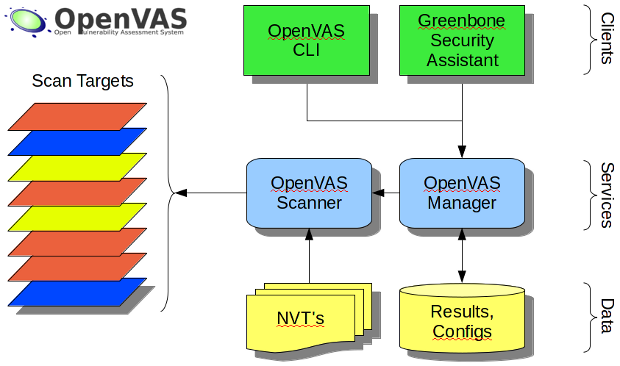
\includegraphics[width=10.0cm]{img/Openvas-structuur.png} \textcite{Openvas-about}
 
De user interface (hierboven vermeld als 'Greenbone Security Assistant') is in veel gevallen een webinterface dat acties doorstuurt naar de manager, zoals een scan starten, of rapporten maken. Het is ook mogelijk om acties door te sturen naar de manager via een command line interface (hierboven vermeld als 'OpenVAS CLI'), dit is handig voor als men scans wil automatiseren.

De manager (hierboven vermeld als 'OpenVAS Manager') staat in voor de communicatie tussen de user interface en de scanner engine. Deze onderhoud ook een database waarin alle configuraties, resultaten, SCAP data, CERT data en NVT's zitten. Het is de job van de manager om deze databank up-to-date te houden zodat deze steeds een volledige vulnerability management oplossing kan bieden.

De scanner (hierboven vermeld als 'OpenVAS Scanner') staat in voor de effectieve scan van een target. Deze heeft een cache waar alle NVT's aanwezig zijn die de scanner nodig heeft om een target te kunnen scannen. Deze geeft zijn resultaten terug aan de manager. 

Indien men een scan start voor een range van machines, zal de scanner engine eerst een 'alive check' uitvoeren op alle hosts in de range. Dit kan bestaan uit een simpele ICMP ping naar de host, tot een range van poorten scannen en kijken of de host reageert op 1 van de requests. 

Indien de host reageert, zal er een port scan gestart worden, de tool die men hiervoor gebruikt is in veel gevallen 'nmap'. De range van poorten wordt op voorhand gedefinieerd door de gebruiker en indien er een firewall aanwezig is, zal hier ook rekening mee gehouden worden. 

De scanner zal hierna een aantal dingen analyseren, zoals het besturingssysteem dat op de host draait, en welke services overeen komen met de open poorten. Als al deze feiten uiteindelijk bekend zijn, zal de scanner op basis van deze analyse NVTs naar de hosts sturen en kijken of deze vatbaar is voor bepaalde exploits \textcite{Qualys}.

Uiteindelijk zal de scanner alle gevonden informatie doorsturen naar de manager, en op basis hiervan een rapport maken die leesbaar is voor de gebruiker.

\subsection{Requirements}

%TODO: wat beter herschrijven
%TODO: functionaliteiten opsommen!

In de volgende delen, zullen we Nessus en Openvas vergelijken op een aantal vlakken dat belangerijk zijn in een scanner. Een aantal belangerijke zaken (snelheid van de scanner, accuraatheid, etc...) zullen pas besproken worden in hoofdstuk~\ref{ch:methodologie}, omdat deze tot mijn onderzoek behoren. Eerst zal er kort een aantal zaken besproken worden zoals de geschiedenis van de scanner, de licenties, de support dat de scanner krijgt en de hardware vereisten. Hierna bespreken we de belangerijkste zaken.

Een volwaardige vulnerabiltiy scanner moet aan een paar voorwarden voldoen, het belangerijkste onderdeel zijn de NVTs. Als deze niet tijdig worden geüpdate, is de scanner niet meer betrouwbaar voor de nieuwste vulnerabilities, en geeft dit een vals veilig gevoel. Hiervoor zullen we 2 grote vulnerabilities (1 voor linux, en 1 voor windows) opzoeken en kijken wanneer beide scanners deze NVT toegevoegd hebben. Voor linux heb ik gekozen voor de 'shellshock' vulnerability (CVE-2014-6271), voor windows is dit 'Server Service Vulnerability' (CVE-2008-4250)

Uiteindelijk bespreken we ook de functionaliteiten van beide scanners. Eerst zullen we bepaalde funtionaliteiten bespreken die een betere performantie geven, of een accurater beeld geven van het systeem. Daarna bespreken we bepaalde functies die niet direct bijdragen tot het eindrapport, maar de scanner gemakkelijker laten implementeren met de bestaande infrastructuur of het grootste deel van het onderhoud automatiseren. 

%TODO: meer testen toevoegen dat impact hebben op eindrapport
Voor het eerste deel gaan we na of beide scanners een 'credential scan' ondersteunen, deze test gebeurt door het inloggen op een bepaalde dienst (meestal ssh) en heeft dus ook de mogelijkheid om configuratie files te controleren op fouten \textcite{Digitalbond}. Een basisvereiste is ook vaak dat scanner meerdere scans tegelijkertijd kunnen uitvoeren, Hoewel dit bij moderne scanners zo goed als steeds het geval is gaan we voor volledigheid dit ook nakijken. Uiteindelijk kijken we ook of de scanner 'agent based' scanning toestaat, dit is een klein programma dat op een host geïnstalleerd word, en commandos van van een centrale machine kan ontvangen. Deze zal een scan uitvoeren op de lokale machine, en zijn resultaten doorsturen naar de centrale machine waar deze beschikbaar is via alle interfaces.

%TOOD: meer testen toevoege ndat GEEn impact hebben op eindrapport 
%TODO: RESP/API uitleggen
Uiteindelijk kijken we of  de server zichzelf onderhoud (zoals NVTs updaten), en wat er nog manueel moet gebeuren. Ook kijken we of er een REST interface, of een API aanwezig is. 
%---------------------------------------------------

\subsection{Nessus}

%TODO: informatie over nessus (prijs,tennable, geschiedenis, edities, support, etc...
%TODO: history citen naar boek V werkt niet voor een reden
%@BOOK{Nessus,
%  TITLE = {Nessus Network Auditing},
%  AUTHOR = {Carey Mark, Russ Roger, Paul Criscuolo, Mike Petruzzi},
%  YEAR = {2008}, 
%  PUBLISHER = {O'reilly},
%}

\subsubsection{Geschiedenis}
Nessus is in 1998 opgericht door Renaud Deraison, met de bedoeling om een gratis vulnerability scanner te maken dat over het internet machines kon scannen. Rond deze software werd het bedrijf tenable opgericht en werd al snel 1 van de populairste oplossingen voor vulnerability managment. Vanaf nessus versie 3 (2005) werd de source code niet meer publiek gemaakt omdat er misbruik van gemaakt werd door de concurrentie. De nessus scanner werd doorverkocht door bedrijven met hun eigen logo en vermelden dat het hun scanner was, ook was er weinig tussenkomst van de community (vooral op gebied van de scanner engine) \textcite{Cnet}.

\subsubsection{Licenties}
Tenable heeft een aantal nessus producten, maar voor deze bachelorproef kijken we naar 'Nessus Professional'. De reden hiervoor is dat dit product zo goed als volledig overeenkomt met een openvas installatie (met een paar limitaties). De licentiekosten hiervoor zijn 2190 \$ / jaar (ongeveer 2010 euro) en is proprietary software.
 
\subsubsection{Support}
Als men een licentie van 'Nessus Professional' heeft, is het mogelijk om support te krijgen via live chat, email en een support portal. Deze zaken zijn 24/7 te benaderen \textcite{Nessus-support}.
 
\subsubsection{Nvt development}
Nessus heeft op moment van schrijven 87.071 plugins \textcite{Nessus-nvt}. Deze NVTS worden geschreven in .nasl (Nessus attack script language).

Voor de shellshock vulnerability is er een NVT verschenen op 24-09-2014 \textcite{Vulners-shellshock-nessus}. Dit is dezelfde dag als shellshock publiek gemaakt werd. De windows vulnerability NVT werd geüpload op 23-10-2008, dit is ook op de dag dat windows de vulnerability publiek maakte.
 

\subsubsection{Functionaliteiten}
\textbf{\textit{Credential scan: }} Deze functionaliteit is beschikbaar, met ondersteuning voor een aantal services. De belangerijste services worden hier opgelijst: database, mongoDB, ssh, windows en SNMPv1/v2c \textcite{Nessus-functions}.

\textbf{\textit{Meerdere scans: }} Dit is mogelijk op elke versie.

\textbf{\textit{Agent based: }} Dit is niet mogelijk met de 'professional' licentie, maar wel met de 'manager' licentie \textcite{Nessus-functions}.
%todo: kijken of nessus cron gebruikt
\textbf{\textit{Onderhoud: }} Op de webinterface is het mogelijk om bepaalde of alle  elementen te updaten. Ook is het mogelijk om een interval in te stellen wanneer deze moet geüpdate worden (dagelijks, wekelijks of maandelijks).

\subsubsection{Hardware}
De minimum systeemvereisten voor een scanner zijn:

\begin{itemize}
\item Dual core 2GHz CPU
\item 2-4 GB RAM
\item 30GB HDD
\end{itemize}

\textcite{Nessus-requirements}

%-------------------------------------------------------------------

\subsection{Openvas}
%%TODO: mailing list uitleggen, IRC?

\subsubsection{Geschiedenis}
Openvas is een fork van de laatste source code die nessus publiek heeft gemaakt (2005), en begon onder de naam \textcite{Securiteam} en werd begonnen door Tim Brown. Dit project is nog steeds volledig opensource \textcite{Openvas-source} en gratis voor zowel personen, als bedrijven met uitzondering op een (niet verplichte) betalende licentie van greenbone voor NVT's \textcite{Openvas-nvt}. De grootste bijdrager voor openvas is greenbone, deze zorgt voor een groot deel van de NVTs, de webinterface en bugfixes \textcite{Openvas-contributors}.

\subsubsection{Licenties}

Openvas valt onder de GPL license, is open-source en is gratis te gebruiken voor zowel personen, als bedrijven.

\subsubsection{Support}
%TODO: monitor IRC chat activity \textcite{Openvas-IRC}.  
Een nadeel van open-source projecten is vaak dat je afhankelijk bent van de community voor support. Dit is bij openvas niet anders, buiten een mailing list is de support zo goed als nietbestaande. De openvas website bevat veel verouderde links zoals een wiki, IRC chat en screenshots. Op het moment van schrijven is de laatste entry in de wiki voor openvas 7 \textcite{Openvas-wiki}, ook op de screenshots pagina is de laatste entry voor openvas 7 \textcite{Openvas-screenshots}.

\subsubsection{Nvt development}
%TODO: worm uitleggen?
Openvas heeft op het moment van schrijven 53.082 plugins \textcite{Openvas-nvt} waarvan er 214 geüpload zijn in de laatste maand. Wat hier ook opvallend is, is dat alle plugins in openvas geschreven worden in nasl (dit staat voor 'nessus attack script language'). Openvas gebruikt dus nog steeds dezelfde code voor NVTs te schrijven als nessus. 

Voor de shellshock vulnerability heeft openvas de NVT geupload op 25-09-2014 \textcite{Vulners-shellshock-openvas}. Dit is 1 dag later als de announcement van shellshock en is gemaakt door greenbone. Dit lijkt onschuldig, maar shellshock heeft 24 uur na de ontdekking al voor het ontstaan van botnets gezorgd \textcite{wired-shellshock}. 

De windows vulnerability werd beschikbaar gesteld op 24-10-2008, Dit is 1 dag na de bekendmaking door windows. Hoewel de gevolgen niet zo erg waren als shellshock, gebruikte de worm \textcite{Microsoft} deze vulnerability om zich te verspreiden.

\subsubsection{Functionaliteiten}
%todo: targets uitleggen?
\textbf{\textit{Credential scan: }} Deze functionaliteit is beschikbaar, maar dit is niet op scan niveau. Dit betekent dat men 2 verschillende targets moet aanmaken als men een credential en een non-credential wil starten (ookal is dit hetzelfde IP). De ondersteunde services zijn hier: SSH, SMB, ESXi en SNMP.

\textbf{\textit{Meerdere scans: }} Dit is mogelijk.

\textbf{\textit{Agent based: }} Dit mogelijk.
%todo: uitleggen wat cron is?
\textbf{\textit{Onderhoud: }} Het is niet mogelijk om in de webinterface updates te starten. De updates (voor alles) worden wel automatisch elke dag geüpdate om 1 uur snachts door middel van cronjobs.

\subsubsection{Hardware}
De minimum systeemvereisten voor openvas staan niet op de site, er is wel een virtuele machine aanwezig voor openvas te testen. De requirements hieronder zijn van deze virtuele machine, in realiteit zullen deze requirements hoger liggen. De reden hiervoor is dat dit een minimale versie is dat bepaalde features niet heeft, ook zijn er nog meer beperkingen zoals dat het besturingssysteem kan niet updaten. Dit is dus niet gepast voor een productie omgeving.

\begin{itemize}
\item Dual core CPU
\item 2 RAM
\item 9GB HDD
\end{itemize}

\textcite{Openvas-requirements}

%-----------------------------------------------------------

\section{Probleemstelling en Onderzoeksvragen}
\label{sec:onderzoeksvragen}

%% TODO:
%% Uit je probleemstelling moet duidelijk zijn dat je onderzoek een meerwaarde
%% heeft voor een concrete doelgroep (bv. een bedrijf).
%%
%% Wees zo concreet mogelijk bij het formuleren van je
%% onderzoeksvra(a)g(en). Een onderzoeksvraag is trouwens iets waar nog
%% niemand op dit moment een antwoord heeft (voor zover je kan nagaan).

\section{Opzet van deze bachelorproef}
\label{sec:opzet-bachelorproef}

%% TODO: Het is gebruikelijk aan het einde van de inleiding een overzicht te
%% geven van de opbouw van de rest van de tekst. Deze sectie bevat al een aanzet
%% die je kan aanvullen/aanpassen in functie van je eigen tekst.

De rest van deze bachelorproef is als volgt opgebouwd:

In Hoofdstuk~\ref{ch:methodologie} wordt de methodologie toegelicht en worden de gebruikte onderzoekstechnieken besproken om een antwoord te kunnen formuleren op de onderzoeksvragen.

%% TODO: Vul hier aan voor je eigen hoofstukken, één of twee zinnen per hoofdstuk

In Hoofdstuk~\ref{ch:conclusie}, tenslotte, wordt de conclusie gegeven en een antwoord geformuleerd op de onderzoeksvragen. Daarbij wordt ook een aanzet gegeven voor toekomstig onderzoek binnen dit domein.

